\documentclass[a4paper,12pt,twoside]{article}

\usepackage{graphicx}
\usepackage{polski}
\usepackage[utf8]{inputenc}
\usepackage{indentfirst}
\usepackage{float}
\usepackage{listings}
\usepackage[scaled]{helvet}
\usepackage{fancyhdr}
\usepackage{pdfpages}
\usepackage[labelsep=period]{caption}
\usepackage{amsmath}
\usepackage{hyphenat}
\usepackage[shortlabels]{enumitem}
\usepackage[titletoc, title]{appendix}
\usepackage{chngcntr}
\usepackage{color}

\renewcommand\familydefault{\sfdefault} 
\usepackage[T1]{fontenc}


\title{Praca inżynierska}
\author{Tomasz Kogowski}

\pagestyle{fancy}
\fancyhf{}
 
\renewcommand{\headrulewidth}{0pt}
\renewcommand{\baselinestretch}{1.15} 

\newcommand{\source}[1]{\caption*{\emph{\footnotesize Źródło elementów graficznych: {#1}.}} }
\fancyfoot[LO,RE]{\thepage}\pagestyle{fancy}

\begin{document}
\includepdf[pages=1]{pierwsza_strona/pierwsza_strona.pdf}
\pagenumbering{arabic}
\newpage 
\section*{Streszczenie}
\newpage 
\section*{Abstract}

\newpage
%\section*{Oświadczenie o autorstwie pracy}
\includepdf[pages=1]{obrazy/oswiadczenie.pdf}
\newpage
\tableofcontents
 
\newpage
\section{Wstęp}  



%Wraz z rozwojem technik uzyskiwania danych z sekwencjonawania DNA, powstało wymaganie stworzenia
%aplikacji, która w prosty i intuicyjny sposób umożliwi lekarzom oraz analitykom analizę ludzkich %genomów.

%W celu osiągnięcia wyżej przedstawionego celu, na Wydziale Elektroniki i Technik Informacyjnych Politechniki Warszawskiej oraz w Warszawskim Instytucie Matki i Dziecka rozpoczeła się praca nad systemem, którego owa praca inżynierska jest częścią.

\subsection{Motywacja}  

\subsection{Cel pracy} 
\newpage
\section{\textcolor{red}{Podstawy teoretyczne}}  

\textit{Czy jest sens pisać o tym? 
1-2 strony o tym czym jest DNA, genomy, kodony, jak zmiana w DNA może wpływać na organizm i dlaczego warto zajmować się badaniem DNA}
\newpage
\section{Wymagania funkcjonalne i niefunkcjonalne}  

%Opisanie o wymaganiu dostępu do próbek oraz transkryptów, 
%filtracji, zapisywaniu wyboru filtrów,
%wyboru widocznych kolumn, sortowania, filtrowania pobranych już danych.

Określenie funkcjonalności dostępnych w budowanej aplikacji, rozpoczęto od określenia 
rodzajów użytkowników, którzy mają korzystać z oprogramowania tak by jak najlepiej dostosować
system do ich potrzeb, przyśpieszyć dostęp do danych.

Pierwszą grupą docelową są lekarze, którzy będą poszukiwali
możliwych chorób powiązanych z wariantem pacjenta, by wykryć niebezpieczeństwa
i móc jak nawcześniej przeciwdziałać chorobom. 
Na dane będą patrzeć w kontekście jednego badanego pacjenta i należy umożliwić Im łatwe 
ich rozróżnienie genotypów. 

Drugim typem są analitycy, którzy będą analizować dane i zadawać 
odwrotne pytania, czyli będą starać się znaleźć warianty, które mogą być odpowiedzialne
za konkretną chorobę. 

Inną istotną kwestią wziętą pod uwagę był typ i wielkość danych, jakie mają być wyświetlane klientom.
W trakcie projektowania architektury jako dane przykładowe zostały wybrane dane dla przykładowego transkryptu dostępne w aplikacji Exac \cite{exac}. Dane te posiadały 36 kolumn i oczywistym wydało się że obie grupy użytkowników będzie interesowała tylko część informacji o genotypie i należało by umożliwić im filtrację oraz zakrywanie niepotrzebnych danych. 
Jedna próbka liczyła sobie więcej niż 340000 wiersze co wymogło zaproponowanie 
funkcjonalności umożliwiającen na poprawne i intuicyjne filtrowanie danych 
tak by klient otrzymywał tylko interesujące go rekordy.

\subsection{Wymagania funkcjonalne}
Po zakończeniu analizy zostały określone następujące funkcjonalności. Aplikacja:

 \begin{enumerate}[1)]
 \item ma wygodny, prosty interfejs użytkownika,
 \item rejestruje użytkowników,
 \item autoryzuje użytkowników,
 \item umożliwia wybór próbki do analizy,
 \item pozwala na wprowadzenie wcześniej zdefiniowanych filtrów z panelu administratora,
 \item wyświetla dane z sekwencjonowania DNA dla konkretnej próbki,
 \item filtruje dane po stronie serwera i wysła je klientowi,
 \item zlicza ilość danych przy zadanych filtrach i informuje klienta o wyniku,
 \item umożliwia zmianę wartości filtrów,
 \item pozwala na wyłączenie z filtracji dowolnej części filtrów,
 \item zapisuje wartości filtrów oddzielnie dla każdego użytkownika,
 \item sortuje dane po stronie klienta,
 \item filtruje dane po stronie klienta,
 \item udostępnia administratorowi możliwość zmiany dostępu do próbek 
 każdego użytkownika
 \item daje możliwość zakrycia na stronie aplikacji części danych	
 \end{enumerate}
 
\newpage
Funkcjonalności umożliwiająca wprowadzanie wcześniej zdefiniowanych filtrów wymusiła stworzenie
trzeciej klasy użytkowników, to jest administratorów, którzy będą zarządzać dostępem do próbek dla 
użytkowników oraz będą wprowadzali plik zmieniający strukturę filtrów.

\newpage
\textit{
Parę wymagań niefukcjonalnych jak dostęp wielu użytkowników na raz, czas odpowiedzi itp.}
\newpage
\section{Istniejące rozwiązania}  

Exac broad institute, Exac Harvard  
Skupić się na tym iż systemy nie pozwalają na personalizacje interfejsu dla użytkownika.
Harvard udostępnia REST API nieprzyjazne użytkownikowi \newline
\textcolor{red}{\textbf{Czy dodać tu zdjęcia z tych aplikacji?}}

\newpage
\section{Wybór technologi}

Platforma klastrowego przetwarzania danych - Apache Spark\cite{spark}, z którą współpracować będzie aplikacja, została stworzona oraz udostępnia interfejs programistyczny w języku Scala.
Naturalnym przez to wydało się wybranie tego języka programowania do stworzenia przeglądarki danych.

  
\subsection{Język programowania Scala}
W aplikacji użyto języka Scala w wersji 2.11.7 \cite{jezykScala}. Jest to język programowania powstały w 2001 roku pod kierownictwem Martina Odersky'ego w Lozannie.
Działa na Wirtualnej Maszynie Javy a do 2012 roku wspierała platformę .NET opracowaną przez firmę Microsoft. Język ten nadaje się równie dobrze do krótkich, zwartych skryptów  wywoływanych podobnie do skryptów języka Python jak i do tworzenia wydajnych, ogromnych, bezpiecznych systemów sieciowych.

Jest językiem łączącym cechy języków funkcyjnych oraz obiektowych. 
Nie jest jednak obligatoryjny fukncyjny styl programowania, do którego nie jest przyzwyczajona większość programistów.
 Scala w swoim założeniu nawiązuje do minimalizmu składni Lispa to znaczy że nie opiera się na składni a na funkcjach bibliotecznych. Nazwa ma podkreślić skalowalność języka, dzieje się tak dzięki możliwości tworzenia dodatkowych typów i struktur wyglądających jak nowa składnia języka.
Zaletą języka jest również to że dzięki kompatybilności z językiem Java mamy możliwość wykorzystania każdej lini kodu napisanej w owym języku.

\subsection{System zarządzania bazą danych}  
Zadanie stworzenia bazy danych przechowującej informacje konfiguracyjne, dane użytkowników oraz o użytkownikach było 
dużą częścią tworzenia systemu i
wymagało wybrania odpowiedniego systemu zarządania bazą danych.
Model bazodanowy został zaprojektowany w modelu opartym na relacyjnej organizacji danych, przez co wybór ograniczył się do
darmowych technologii realizujących relacyjne bazy danych.

\newpage
Biorąc pod uwagę powyższe kryteria, można porównać najpopularniejsze systemami, są nimi\cite{porownanieBaz}: 
 \begin{itemize}
  \item MqSQL
  \item SQLite
  \item PostgreSQL
\end{itemize}

\subsubsection{MySQL}
\paragraph{Zalety}
\begin{itemize}
\item{proste i łatwe w obsłudze}
\item{wysoki poziom bezpieczeństwa}
\end{itemize}
\paragraph{Wady}
\begin{itemize}
\item{nie realizuje w pełni standardu SQL}
\item{problematyczny jednoczesny zapis i odczyt}
\end{itemize}
\subsubsection{SQLite}
\paragraph{Zalety}
\begin{itemize}
\item{zgodny ze standardem SQL}
\item{przenośny dzięki oparciu bazy o jeden plik}
\end{itemize}
\paragraph{Wady}
\begin{itemize}
\item{brak zarządzania użytkownikami i dostępami do danych}
\end{itemize}

\subsubsection{PostgreSQL}
\paragraph{Zalety}
\begin{itemize}
\item{zgodny ze standardem SQL}
\item{wsparcie dla współbieżności}
\item{pełne wsparcie dla transakcji}
\end{itemize}
\paragraph{Wady}
\begin{itemize}
\item{słaba wydajność}
\item{trudność instalacji dla początkujących użytkowników}
\end{itemize}

\subsubsection{Uzasadnienie wyboru PostgreSQL}
Po analizie ostateczny wybór systemem padł na PostgreSQL.
To otwarte i darmowe oprogramowanie posiada bardzo dużą społeczność, której wiedza jest łatwo dostępna w internecie 
i posiada wiele narzędzi i bibliotek przeznaczonych do pracy z owym systemem. 
Istotny wpływ na decyzje miała również łatwość integracji PostgreSQL na inne systemy.  

\subsection{Slick}  
Pracę z bazą danych po stronie serwera aplikacyjnego 
znacznie ułatwia oprogramowanie pozwalające na odwzorowanie obiektowo-relacyjne tabel bazodanowych na obiekty języka programowania.
Dzięki tej technice programista może traktować obiekty bazodanowe jak elementy kolekcji czy pola obiektów.

Takim narzędziem jest stworzone przez firmę Lightbend, Inc. 
oprogramowanie Slick\cite{slick} pozwalające na pełną kontrolę nad bazą danych oraz pisanie klasycznych zapytań SQL.


\subsection{Aplikacja przeglądarkowa}
Biorąc pod uwagę wymagania klientów oraz różnorodność używanych przez nich urządzeń należało wybrać odpowiedni rodzaj aplikacji klienckiej pozwalający na spełnienie wszystkich wymagań funkcjonalnych naszych użytkowników 
oraz jednocześnie będący łatwy w utrzymaniu i rozwijaniu.

\paragraph{Zalety aplikacji internetowych}
Łatwość w dostępie do internetu, ilość urządzeń pozwalających na 
korzystanie z przeglądarek internetowych pozwoliły 
na rozwój aplikacji internetowych oraz ich rozpowrzechnienie.
Łatwość w rozbudowie, zarządzaniu i 
niskie ceny hostowania serwera aplikacyjnego spowodowały 
powstanie grupy platform programistycznych wspomagających ich budowę. 

Narzędzia typu Ruby on Rails czy Spring Boot 
zdejmują z programisty obowiązek konfiguracji serwera 
HTTP od podstaw i umożliwiają rozpoczęcie pracy  
nad stronami aplikacji po kilku minutach.

\paragraph{Platforma programistyczna Play}
Platforma Play, stworzona w języku Scala jest środowiskiem 
do tworzenia aplikacji internetowych, 
która na celu ma przyśpieszyć pracę programisty dzięki:
\begin{itemize}
\item strategii Konwencji Ponad Konfigurację
\item przeładowywania i ponownej kompilacji plików po edycji
\item wykorzystaniu wzorca Model-Widok-Kontroler
\item wykorzystaniu technologii REST
\end{itemize} 
  
\newpage
\section{Przypadki użycia}

\textcolor{red}{Czy skupić się bardziej na opisie działania aplikacji czy raczej implementacji?}

\subsection{Autoryzacja}
\subsubsection{Role}
\subsubsection{Rejestracja użytkownika}
\subsubsection{Logowanie użytkownika}

\subsection{Przeglądanie danych z sekwencjownowania DNA}
\subsubsection{Widok listy dostępnych próbek}
\subsubsection{Ekran dostępnych genomów}
\subsubsection{Filtrowanie danych}

\subsection{Panel administratora}
\subsubsection{Zarządzanie filtrami}
\subsubsection{Zarządzanie rolami użytkowników}
\subsubsection{Zarządzanie widocznością próbek dla użytkowników}

\newpage
\section{Schemat bazy danych}
\textcolor{red}{
Schemat jest bardzo duży, może załączyć w częściach w dodatku i odsyłać tam czytelnika?
}
\begin{figure}[h!]
  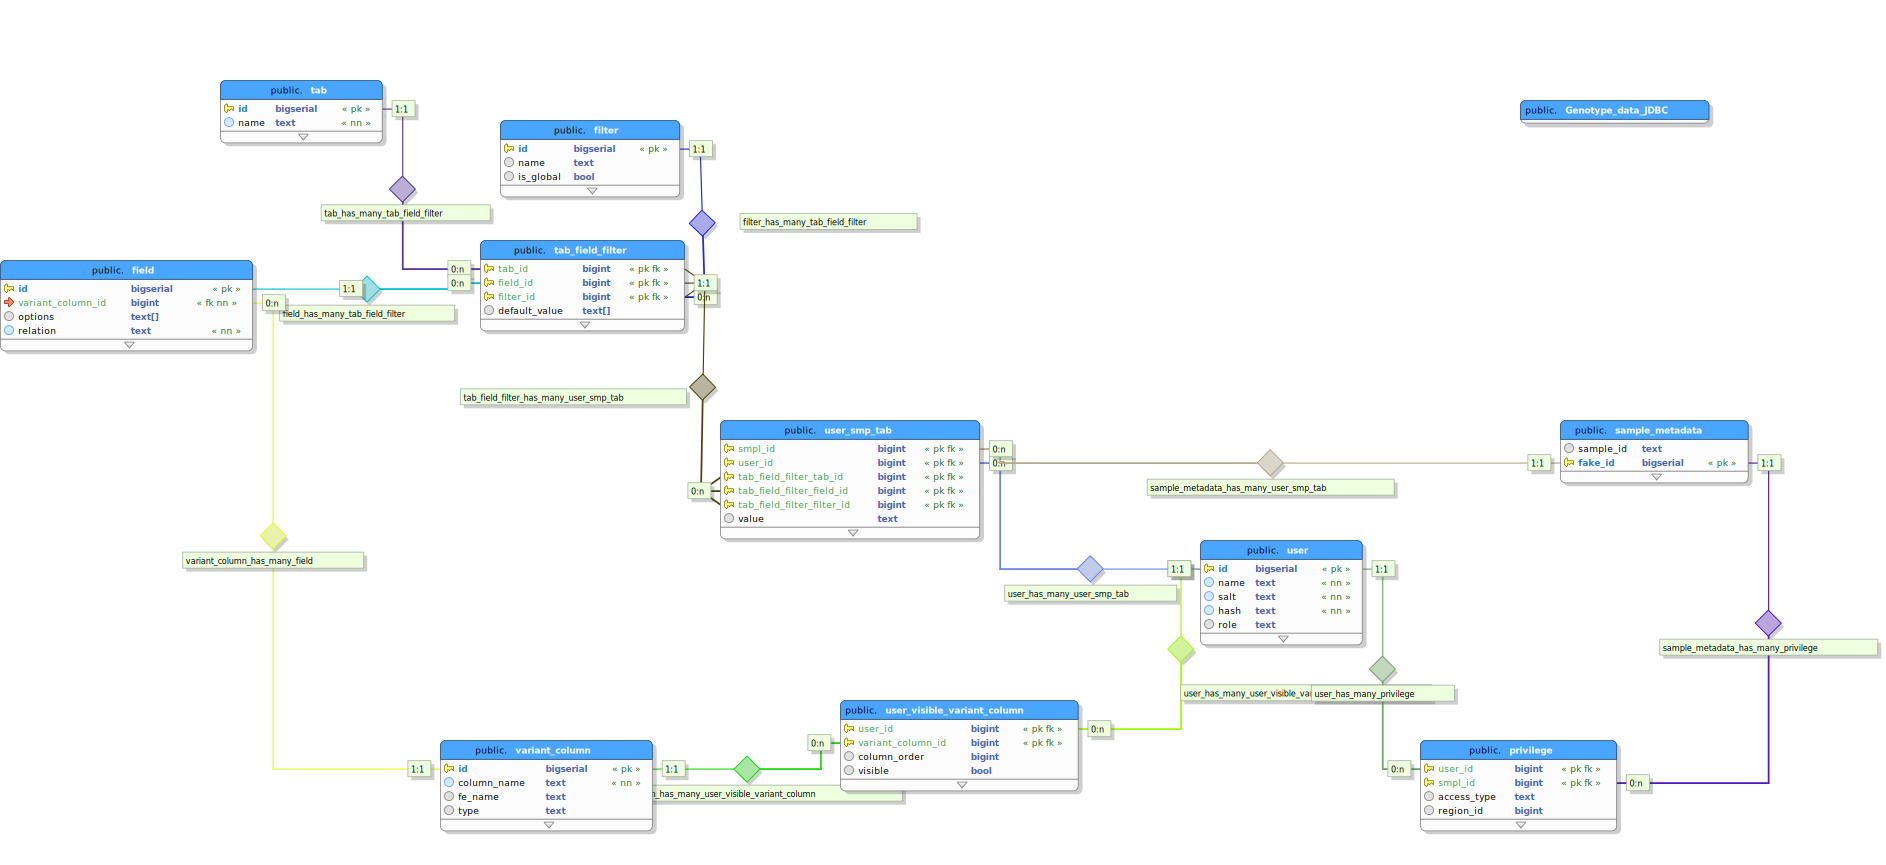
\includegraphics[width=\linewidth]{obrazy/database.png}
  \caption{Schamat bazy danych}
  \label{fig:bazadanych}
\end{figure}

\newpage
\section{Opis implementacji}  
\textcolor{red}{
Czy nie połączyć opisu implementacji razem z przypadkami użycia?
Kolejno opisując użycie aplikacji mógłbym opisać jak to się odbywa w kodzie.
}
\newpage
\section{Bezpieczeństwo aplikacji}  
\subsection{Niebezpieczeństwa}
\subsection{Wykorzystanie protokołu https}
\textit{Opisać jak od strony bardziej technicznej odbywa się zabezpieczanie haseł użytkownika (sól, sha512) }
\newpage
\section{Testy oraz wydajność}  
\newpage
\section{Wnioski i podsumowania}  

\addcontentsline{toc}{section}{Literatura}
\newpage
\begin{thebibliography}{99}

\bibitem{jezykScala}
École Polytechnique Fédérale - Scala documentation,
Available at: http://docs.scala-lang.org/ (Accessed: 10 August 2017).

\bibitem{spark}
The Apache Software Foundation - Apache Spark Available at: https://spark.apache.org/ (Accessed: 10 August 2017).

\bibitem{exac}
Exac Browser Data - Exome Aggregation Consortium  
Available at: http://exac.broadinstitute.org/ (Accessed: 10 August 2017).

\bibitem{porownanieBaz}
Hostovita sp. z o.o. - Porównanie relacyjnych SZBD: SQLite, MySQL, PostgreSQL
Available at:
https://hostovita.pl/blog/porownanie-relacyjnych-systemow-zarzadzania-bazami-danych-sqlite-mysql-postgresql/ (Accessed: 10 August 2017).

\bibitem{slick}
Lightbend, Inc Slick documentation. Available at:
http://slick.lightbend.com/docs/ (Accessed: 10 August 2017).
\end{thebibliography}

\newpage
\section*{Wykaz rysunków i tabel} 
\end{document}